% ~ 12 pages
\chapter{Identification of Hadronic Tau Lepton Decays using Neural Networks}
\label{sec:rnn}

This chapter investigates the application of neural networks for tau
identification. First it will be shown that a simple multi-layer perceptron
(MLP) can achieve a classification performance comparable to the optimised BDT
from the previous chapter. Subsequently, novel sequence learning techniques are
employed to create classifiers operating on sequences of reconstructed objects.
For this the recurrent neural networks based on the LSTM architecture are used
to create classifiers operating on tracks in the inner detector and clusters in
the calorimeter. In this context a tau identification algorithm using purely
calorimeter information is developed and its potential application for reducing
the trigger-rate of a di-tau trigger at the \emph{High Luminosity LHC} (HL-LHC)
is presented. Finally, a model combining the multi-layer perceptron and the
recurrent networks operating on track- and cluster-information is developed.

\todo[inline]{Same samples as BDT-ID (except HL-LHC).}

\section{Identification using Feedforward Neural Networks}
\label{sec:ffnn_id}

Before proceeding to sequence classification techniques the viability of neural
networks to perform tau identification using simple network architectures is
shown. This will aid as a introduction to important concepts when training
neural networks. Moreover, the resulting network will be used as a building
block in the final model.

The optimised BDT from Chapter~\ref{sec:bdt} will be used as a reference for the
investigations in this chapter. Therefore the models will be trained and
evaluated using the same event samples, preselection and reweighting scheme
presented in Section~\ref{sec:bdt_eventsim}. In contrast to hold-out validation
used in the previous chapter, the full event sample is now randomly split into a
training, validation and testing sample. The samples have a relative size of
\SI{40}{\percent}, \SI{10}{\percent} and \SI{50}{\percent}, respectively. The
purpose of the training and testing sample is the same as before, however the
validation sample is monitored during the training process and used to perform
model selection and early stopping. A separate sample, as opposed to the testing
sample, is used to avoid introducing biases in the performance measurement on
the testing sample.

A multi-layer perceptron with two hidden layers~(cf.\
Section~\ref{sec:nn_feedforward}) is used

rectified linear units (ReLU)

- Same input variables \& same transformations
- Train, Validation, Test split of \SI{40}{\percent} - \SI{10}{\percent} - \SI{50}{\percent}
- Validation set monitored during training (but not used for training) to stop training early when no improvements in validation loss are observed (using testing set would introduce bias)
- Additionally standardisation is applied (subtract mean and divide by standard deviation) -- important to get a working network (feature scaling)
- Dense layers with ReLU activation
- binary cross entropy loss function (backref)
- Comparison with BDT-based ID

\todo[inline]{Explain the reason for the train-validation-test split. 50-10-40.
  Validation is used for model selection, while testing is used to give final
  performance results. This procedure will be used for the remainder of this
  thesis.}

\todo[inline]{ROC-Curves comparing BDT ID and MLP ID. Make reference dashed to
  see the MLP curve.}

\todo[inline]{How does the performance depend on the size of the sample (this
  would be very interesting to see)}
\section{Identification using Recurrent Neural Networks}
\label{sec:rnn_id}

\subsection{General Description}
\label{sec:rnn_descr}

\begin{figure}[ht]
  \centering
  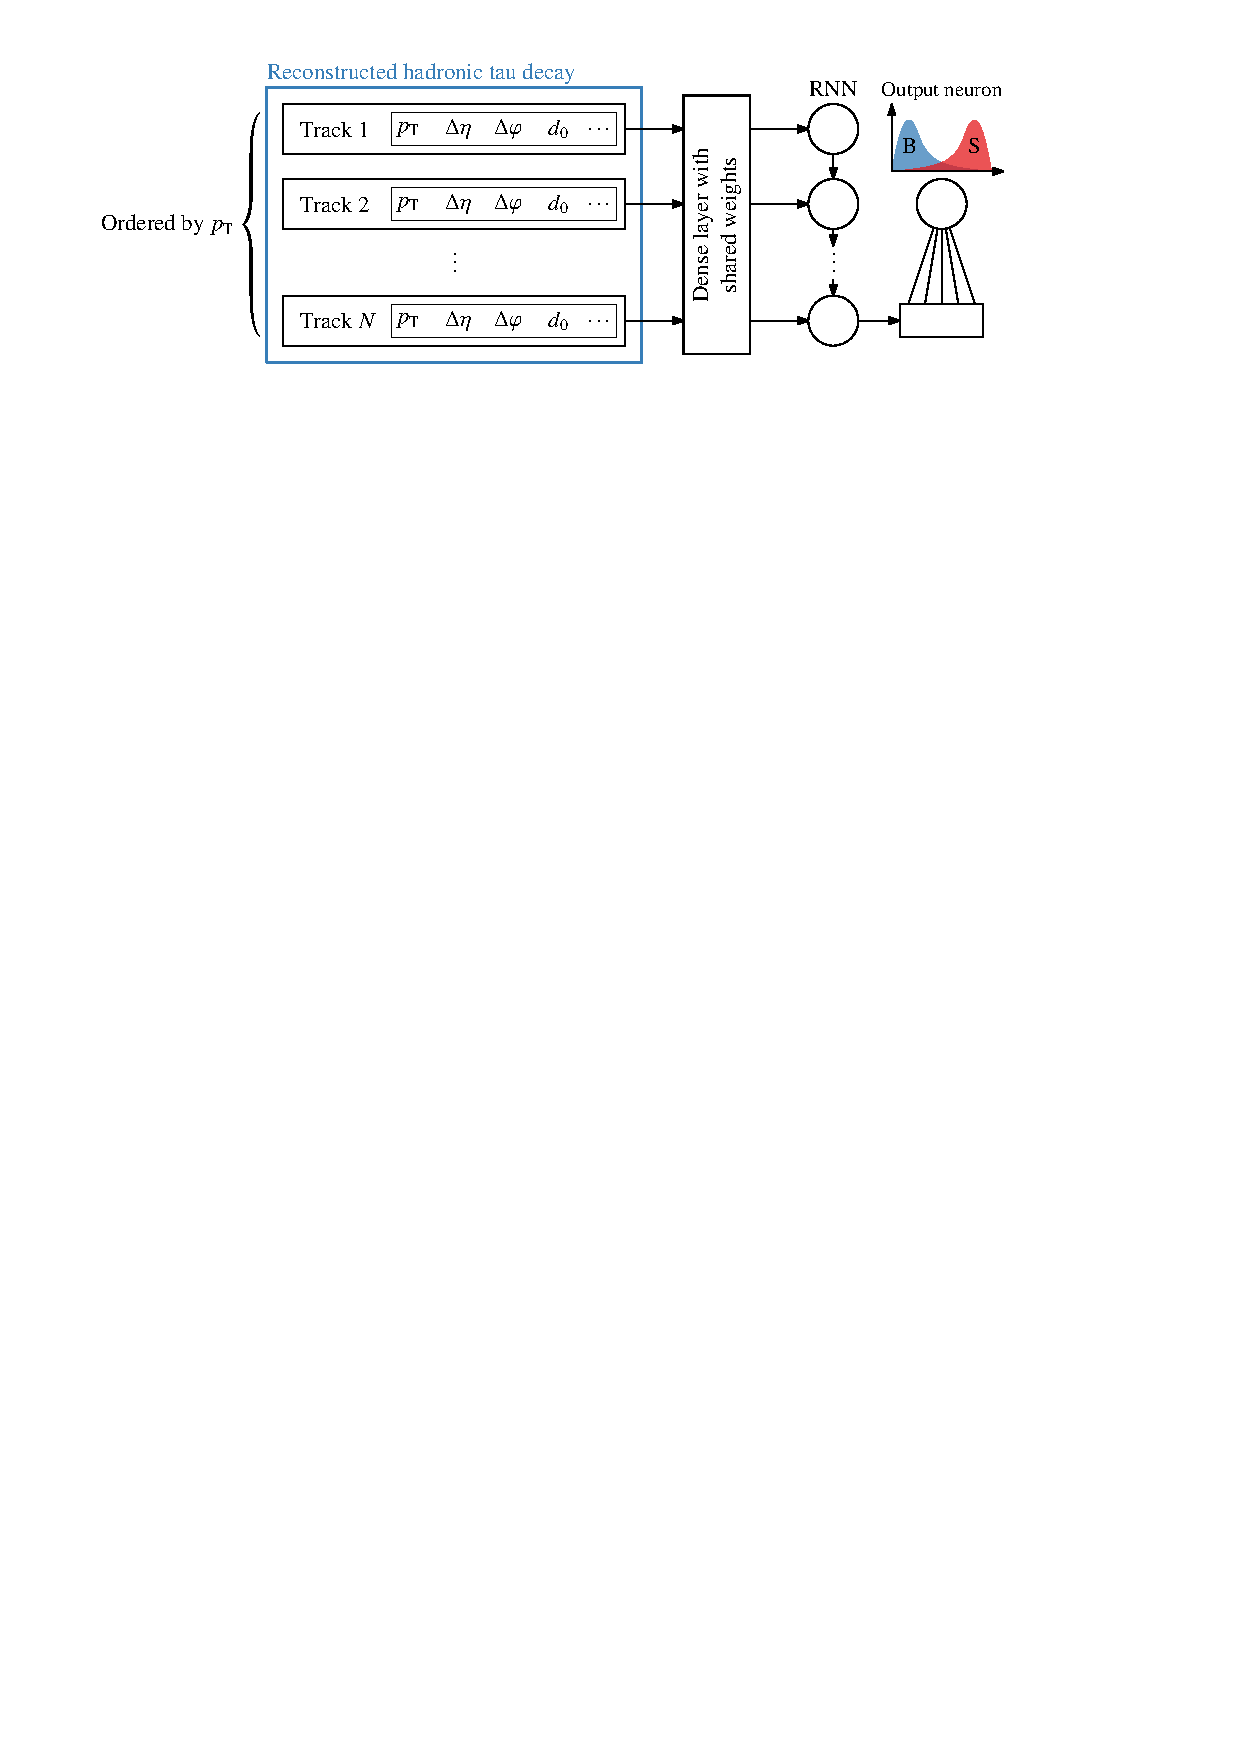
\includegraphics{./figures/rnn/track_rnn_schematic.pdf}
  \caption{Schematic of the Track-RNN}
  \label{fig:track_rnn_schematic}
\end{figure}

State that the RNN is mainly optimised for 1-prong operation and give reasons
for that (i.e.\ higher branching ratio)

\todo[inline]{Correlation with output / label}
\todo[inline]{Group-wise variable importances for RNN}
\todo[inline]{LSTM cell size scan $n_c \in \{8, 16, 24, 32, 48, 64\}$}

\subsection{Track-RNN}
\label{sec:rnn_tracks}

\todo[inline]{ROC-Curves}

\todo[inline]{Check whether the missing tau hits in the ID are a problem at
  high-pt.}

Using reconstructed tracks with a minimum transverse momentum of
\SI{400}{\mega\electronvolt} (already applied in track reconstruction).

Input Variables: Transverse momentum of the track $p_\text{T}^\text{track}$
measured in the tracking system; Absolute value of the transverse impact
parameter $d_0$ with respect to the associated vertex; Distance of closest
approach to the primary vertex in the $z$-$r$ plane $z_0 \sin\theta$ where
$\theta$ is the polar angle of the track \todo{Axis is corrected, use
  $\sin\theta$ instead of $z_0$ due to expected larger error in forward
  direction}; Signed angular distance of track and tau axis $\Delta \eta$ and
$\Delta \varphi$; Electron probability from high-threshold hit information in
the TRT $p_\text{HT}$; Number of hits in IBL $N_\text{hit}^\text{IBL}$, the
three pixel layers (B-layer, 1 and 2) $N_\text{hit}^\text{pixel}$ and the SCT
$N_\text{hit}^\text{SCT}$ (dead sensors crossed by the reconstructed track are
also counted as hits).

Variable importances:
\begin{enumerate}
\item $d_0$ and $z_0 \sin\theta$
\item $p_\text{T}^\text{track}$ and $p_\text{T}^\text{jet}$
\item $\Delta \eta$ and $\Delta \varphi$
\item \texttt{nInnermostPixelHits}, \texttt{nPixelHits} and \texttt{nSCTHits}
\item \texttt{eProbabilityHT}
\end{enumerate}

\begin{table}[ht]
  \centering
  \begin{tabular}{p{5cm}S[table-format=1.4(4)]S[retain-explicit-plus, table-format=+2.1]}
  \toprule
  {Variables} & {Validation loss} & {Loss increase} \\
  \midrule
  \parbox[c]{\hsize}{Impact parameter \newline $d_0$, $z_0 \sin\theta$}
          & 0.2831 +- 0.0005 & + 48.4 \,\si{\percent} \\[1.2em]
  \parbox[c]{\hsize}{Transverse momentum \newline $p_\text{T}^\text{track}$, $p_\text{T}^\text{jet}$}
          & 0.2410 +- 0.0007 & + 26.3 \,\si{\percent} \\[1.2em]
  \parbox[c]{\hsize}{Angular distance \newline $\Delta \eta$, $\Delta \varphi$}
          & 0.2304 +- 0.0003 & + 20.8 \,\si{\percent} \\[1.2em]
  \parbox[c]{\hsize}{Hits in ID \newline $N_\text{hit}^\text{pixel}$, $N_\text{hit}^\text{SCT}$}
          & 0.2036 +- 0.0013 & + 6.7 \,\si{\percent} \\[1.2em]
  \parbox[c]{\hsize}{Electron probability (TRT) \newline $p_\text{HT}$}
          & 0.1930 +- 0.0004 & + 1.2 \,\si{\percent}\\
  \bottomrule
\end{tabular}

%%% Local Variables:
%%% mode: latex
%%% TeX-master: "../mythesis"
%%% End:

  \caption{Variable importance table}
\end{table}

\todo{use 10 tracks}

\todo{LSTM cell size scan? 8, 12, 16, 24, 32, 48, 64}

\todo{Variable importance (in groups?)}

\todo{\SI{40}{\percent} training, \SI{10}{\percent} validation and \SI{50}{\percent} testing}

What has been tested:
\begin{itemize}
\item Ordering $p_\text{T}$
\item Preprocessing
\item Variables: Track classification
\item
\end{itemize}

\begin{figure}[ht]
  \begin{subfigure}[t]{0.48\textwidth}
    \centering
    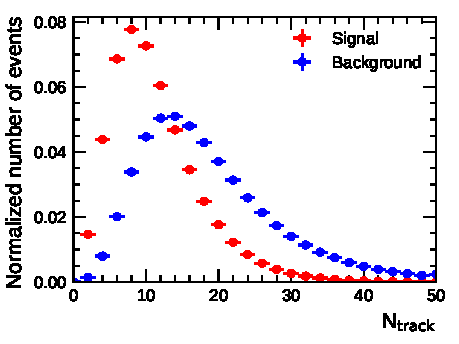
\includegraphics{./figures/rnn/ntrk_1p.pdf}
    \subcaption{NTracks for 1-prong taus. The reco.\ three prong distribution is
      similar with the difference being that at least three tracks are
      required.}
  \end{subfigure}\hfill
  \begin{subfigure}[t]{0.48\textwidth}
    \centering
    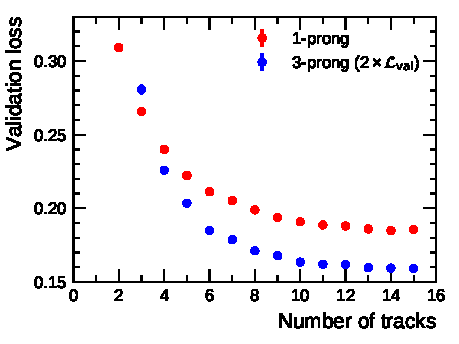
\includegraphics{./figures/rnn/nscan/track_1p_3p.pdf}
    \subcaption{Val.\ loss vs.\ nTracks. Errors are of the
      order of the marker size.}
  \end{subfigure}
  \caption{Tracks associated with a tau}
  \label{fig:rnn_ntracks}
\end{figure}

\begin{itemize}
\item Motivation (i.e. \texttt{SumPtTrkFrac} \& MVA-tracking)
\item Architecture (mention rough optimisation by hand while monitoring
  validation loss)
\item Preprocessing
\item Input variables \& correlation with true (or predicted?) class labels.
  Partial dependence plots? Variable importance?
\item Standalone performance vs. BDT-based ID
\end{itemize}

\begin{itemize}
\item Validation loss vs.\ sample size
\end{itemize}

\subsection{Cluster-RNN}
\label{sec:rnn_clusters}

\todo[inline]{ROC-Curves}

\todo{Idea is to use cluster moments as a proxy for cell-based variables}

Variable evolution:
\begin{itemize}
\item Energy fractions in PS, EM1, EM2, EM3 (only small improvement)
\item $\Delta R \rightarrow \Delta \phi, \Delta \eta$
\item Importance: 1.\ Direction of the cluster $\Delta \phi, \Delta \eta$; 2.\
  Energy and pt of the jet; 3.\ Cluster moments; 4.\ Energy fractions
\end{itemize}

\begin{figure}[ht]
  \begin{subfigure}[t]{0.48\textwidth}
    \centering
    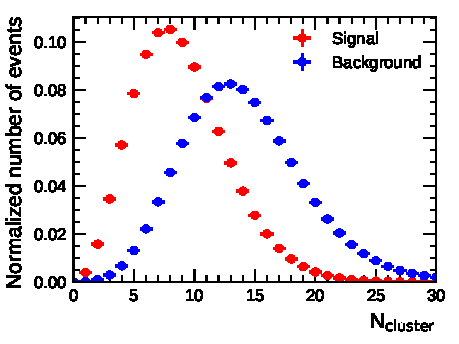
\includegraphics{./figures/rnn/ncls_1p.pdf}
    \subcaption{NCluster for 1-prong taus}
  \end{subfigure}%
  \begin{subfigure}[t]{0.48\textwidth}
    \centering
    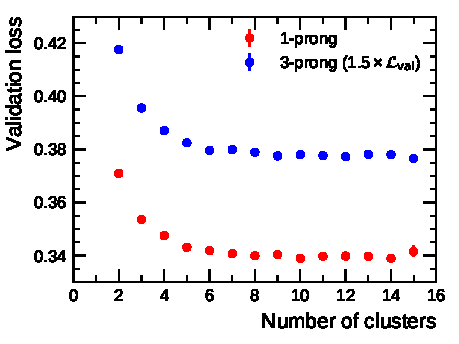
\includegraphics{./figures/rnn/nscan/cluster_1p_3p.pdf}
    \subcaption{Val.\ loss vs.\ nCluster}
  \end{subfigure}
  \caption{Clusters associated with a tau}
  \label{fig:rnn_nclusters}
\end{figure}

\todo{Use 6 clusters}

\begin{itemize}
\item Input variables \& correlation with true class labels. Partial
  dependence plots?
\item Validation loss vs. number of clusters
\item Standalone performance
\end{itemize}

\subsubsection{Rate-Reduction at the High Level Trigger}
\label{sec:hlt_rate_reduction}

Extended barrel to~$\eta = \num{4.0}$. JZ0W sample \todo{cross section} and
Ztautau sample with~$\mu = \num{200}$ and $\sqrt{s} = \SI{14}{\TeV}$. Offline
reconstruction using Run-II calibrations -- i.e.\ not optimised for HL-LHC
conditions (shitty energy calibration -- thats why plots are vs.\ truth pt)

\begin{figure}[htb]
  \centering
  \begin{subfigure}[t]{0.48\textwidth}
    \centering
    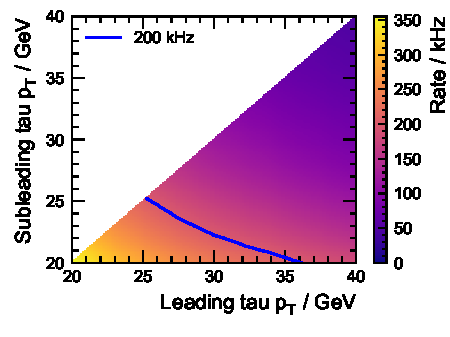
\includegraphics{./figures/rnn/trigger/pt_rate_reg.pdf}
    \subcaption{Rate JZ0W as a function of thresholds}
  \end{subfigure}\hfill
  \begin{subfigure}[t]{0.48\textwidth}
    \centering
    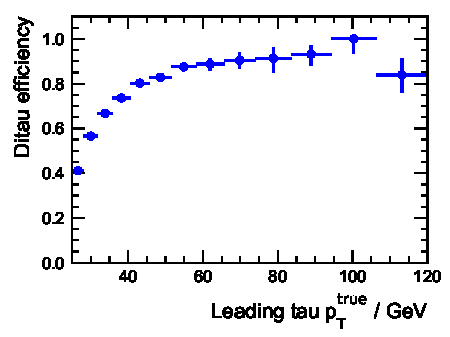
\includegraphics{./figures/rnn/trigger/taueff_reg.pdf}
    \subcaption{Di-tau efficiency}
  \end{subfigure}
  \caption{Di-tau trigger}
  \label{fig:rnn_ditau_trigger}
\end{figure}

The high rates of the High Level Trigger (HLT) for tau leptons need to be
reduced. At the HLT no track information is available due to the high time
requirements of the ATLAS tracking algorithm. The rate reduction is limited to
calorimeter-based variables.

HL-LHC \cite{hl_lhc}. Target rate \SI{200}{\kilo\hertz} from average bunch
crossing rate \SI{31.6}{\mega\hertz}.

\subsection{Combined-RNN}
\label{sec:rnn_combined}

\todo[inline]{ROC-Curves}


\begin{itemize}
\item Architecture
\item Performance w.r.t. BDT-ID
\item ROC of Track+Cluster \& Track+Cluster+IDvars
\item 3-prong cannot achieve Tau-ID level: Secondary vertex determination and
  invariant mass difficult
\end{itemize}

\todo[inline]{Study pile-up dependency of RNN vs BDT-ID}

%%% Local Variables:
%%% mode: latex
%%% TeX-master: "mythesis"
%%% End:
